\chapter{State of the art and background} \label{}
This chapter presents an in-depth review of current and related works,
presenting a general overview of interactive evolutionary computation and their
evolution in the pass and recent years, also user model approaches, In the same
way some works were review that contain the fuzzy logic concept and finally
gamification paradigm is also reviewed.

\section{Interactive Evolutionary Computation.}

This technology is a branch of Evolutionary Computation (EC). 
Based on subjective human
evaluation. Basically, this technique requires that the objective function is
replaced by a person (user) [12].%% What is this?? Please add references correctly
Takagi defines it as "An optimization
technology that uses human evaluation in the optimization system instead of a
human evaluation model". Simply stated, an Interactive EC system() 
is an EC whose fitness function is replaced by a human.  
In figure \ref{fig:IEC} we show a general IEC system.

\begin{figure*}
	\captionsetup{justification=centering,margin=2cm}
	\centering
	\setlength\fboxsep{0pt}
	\setlength\fboxrule{0.7pt}
	\fbox{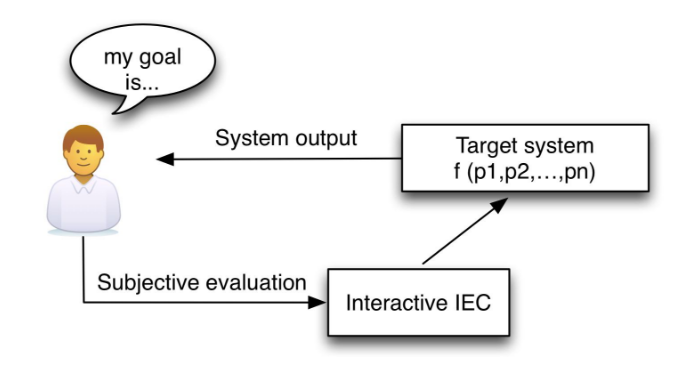
\includegraphics[width=10cm,height=10cm,keepaspectratio]{img/IECGeneral.png}}
	\caption{ General Interactive Evolutionary Computation system based on subjective evaluation.}
	\label{fig:IEC}
\end{figure*}



In this general IEC system we note that the user replaced the fitness function
at the moment he or she interacts with the system. The user could have a
goal that allows him or her to perform the evaluation. Finally
users receive a new output from the system and start over again.

Dawkins\'s research was the pioneer  the
1990s IEC algorithms research works\cite{dawkins1986blind}.

There are two key research approaches in this field:

\begin{itemize}
	\item \textbf{Creative Approach:} The Artificial Life (AL) was the base of the
	creative approach. AL uses complex algorithms for biological life models
	emulation. To perform this task, it is needed to include some of the different
	techniques starting from right image treatment. Good graphic creation as well
	as a great music and
	quality sounds, \cite{sims1991artificial}, \cite{sims1994evolving},
	\cite{dawkins1986blind}, \cite{disz1997ubiworld},
	\cite{unemi2000sbart}and \cite{unemi2003sbeat3}.
	\item \textbf{Humanized technology approach:} The concept of humanized
technology approach comes from the approach that is focused on the IEC
algorithms interface, this is the research of interaction between humans and
computer systems. The main goal of this was to reduce the user's fatigue and to
promote the inputs and outputs of algorithms to improve the efficiency of them.
IEC has made his own way in practical fields such as engineering,
education,etc.,
	\cite{parmee1993concrete}, \cite{ventrella1994explorations},
	\cite{takagi1996discrete}, \cite{poli1997genetic},
	\cite{parmee1998genetic} and \cite{takagi1998interactive}.
\end{itemize}




Computer graphics (CG) The Biomorph of Dawkins was the first IEC research, from
this research comes to many motivated works mostly about the Selfish Gene, come
of these works are:  \cite{ochoa1998genetic},
\cite{mccormack1993interactive}.

In Dawkins work, a conventional recursive algorithm was used as a baseline
maintaining the main target of trees with an L-system (Lindenmayer). This same
L-system was the base for another experiment to create 2-D CG forms insects from
a system called Blind Watchmaker who used L-system angles from L-system output
intuitively selected; the creation was called biomorphs. These creations reach
his target with the multiple selections of the users based on their preferences;
all these selections acted like a natural adaptation filter.

We can find plenty of applications and works for fractal generation and
\cite{sims1992interactive}, \cite{baluja1993simulating} and
\cite{baluja1994towards}, \cite{lund1995artistic}, or
\cite{angeline1996evolving},\cite{raynal1999manipulation}[Raynal 1999] and
\cite{lutton2003artie}, for rendering in tridimensional,
\cite{todd1992artificial},\cite{broughton1997use}, \cite{das1994genetic}[Das
1994] and \cite{tam2002genetic}, for generation of virtual creatures,
\cite{rowland2000evolutionary}, or aerodynamic surface design (wings),
\cite{nguyen1993evolvable}, \cite{nguyen1994evolvable}.

We can discover more than one additional way to use this research in the
artistic field with several applications of IEC who are used for cartoon face
construction and animations matters, like Mutator \cite{todd1994evolutionary}
and \cite{todd1999mutation} or \cite{bentley1999introduction}.

The genetic programming (GP) applications offers a category called Interactive
Genetic Programming (IGP) with many examples of successful application in
tridimensional artwork for artistic animations or construction using
mathematical equations as CAVE \cite{das1994genetic},
\cite{papka1996ubiworld} and \cite{disz1997ubiworld},
\cite{sims1991artificial},
\cite{sims1992interactive} and \cite{min2004creative}. As
this work consequence, Panspermia or Primordial Dance was created that are
presented in figure \ref{fig:Panspermia} and figure \ref{fig:PrimordialD}.

\begin{figure*}
\captionsetup{justification=centering,margin=2cm}
\centering
\setlength\fboxsep{0pt}
\setlength\fboxrule{0.7pt}
\fbox{
\includegraphics[width=10cm,height=10cm,keepaspectratio]{img/Panspermia.png}}
\caption{Panspermia.}
\label{fig:Panspermia}
\end{figure*}

\begin{figure*}
\captionsetup{justification=centering,margin=2cm}
\centering
\setlength\fboxsep{0pt}
\setlength\fboxrule{0.7pt}
\fbox{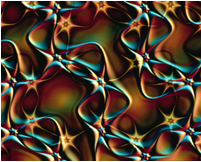
\includegraphics[width=10cm,height=10cm,keepaspectratio]{img/PrimordialDance.png}}
\caption{Primordial Dance.}
\label{fig:PrimordialD}
\end{figure*}


The artistic field is only the first step of a great IEC implementation; it is
important to mention another relevant projects called Galapagos,
\cite{sims1997interactivity}, and SBART, \cite{unemi2000sbart}. The IEC
application Galapagos Project is the exhibit in Tokio Multimedia Museum, (NTT
Intercommunication Center) and this project originates engaging images to all
visitors based on L-systems as we can see in figure \ref{fig:Galapagos1} and
figure \ref{fig:Galapagos2}.

\begin{figure*}
\captionsetup{justification=centering,margin=2cm}
\centering
\setlength\fboxsep{0pt}
\setlength\fboxrule{0.7pt}
\fbox{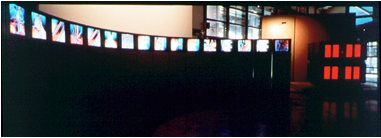
\includegraphics[width=10cm,height=10cm,keepaspectratio]{img/Galapagos1.png}}
\caption{Galapagos: Tokio Multimedia Museum.}
\label{fig:Galapagos1}
\end{figure*}

\begin{figure*}
\captionsetup{justification=centering,margin=2cm}
\centering
\setlength\fboxsep{0pt}
\setlength\fboxrule{0.7pt}
\fbox{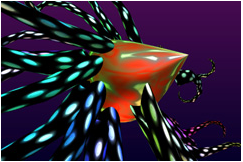
\includegraphics[width=10cm,height=10cm,keepaspectratio]{img/Galapagos2.png}}
\caption{Galapagos' output sample.}
\label{fig:Galapagos2}
\end{figure*}

There are created after one selection, to get a good solution through multiple
repetitions. This action is performed with Genetic Programming (GP), after the
calculation of each pixel value using trees of equations combining logarithm,
maximum, and minimum, sine, root, cosine, exponential arithmetic operators.
AnimationLab is found as an outstanding work who offer figures that can run or
walk working with the user to receive more opportunities to be picked. A
particular characteristic of all of the figures is that the figures extremities
Mentioning open source works, we can find SBART as an IGP
\cite{unemi2000sbart} tool to create graphics. SBART allow to users
to evaluate 20 two-dimensional images, subsequently twenty new image has
direction and angles as we can see in figure \ref{fig:AnimationLab}.

\begin{figure*}
\captionsetup{justification=centering,margin=2cm}
\centering
\setlength\fboxsep{0pt}
\setlength\fboxrule{0.7pt}
\fbox{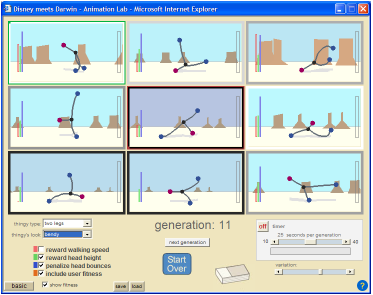
\includegraphics[width=10cm,height=10cm,keepaspectratio]{img/AnimationLab.png}}
\caption{Animation Lab.}
\label{fig:AnimationLab}
\end{figure*}

There are many examples for this field application as
\cite{mckenna1990dynamic},
\cite{ventrella1994explorations}, or
\cite{ventrella1995disney}, \cite{lim1999pro} and
\cite{lim2000solve}.  One of the Interactive Evolutionary Programming
(IEP)  artistic application was created by \cite{angeline1996evolving}, as a fractal generation where the system allows the evolution of
animations for the ones who were selected from the user, the application
initially show only 10 animations to rate.


It is important to know how IEC was implemented in music generation, with
several applications in this field. We will start mentioning the pioneer
application GENJAM, \cite{biles1994genjam},
\cite{biles1996neural} or \cite{biles1999life} and
\cite{biles2002genjam}. Some other attractive works are Sonomorph,
\cite{nelson1993sonomorphs} and \cite{nelson1995further}, or SBEAT, \cite{unemi2003sbeat3},
\cite{horowitz1994generating}, \cite{onisawa2000composition}, \cite{tokui2000music} and
\cite{fels2002interactive}. It is possible to hear a part of the
music songs of these previously mentioned works broadcasted in the radio station
WDYN. (100.1, New York, USA, WEBPage:http://www.wdyn.net/).

The IEC algorithms are the base for the functionality of the music generation
systems, a visual representation of this is given in the below figure \ref{fig:GENJAM}:

\begin{figure*}
\captionsetup{justification=centering,margin=2cm}
\centering
\setlength\fboxsep{0pt}
\setlength\fboxrule{0.7pt}
\fbox{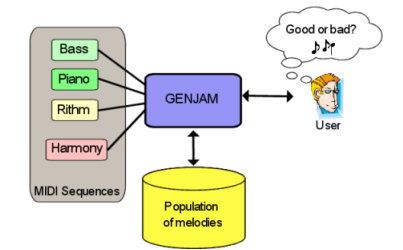
\includegraphics[width=10cm,height=10cm,keepaspectratio]{img/GENJAM.png}}
\caption{GENJAM squeme.}
\label{fig:GENJAM}
\end{figure*}

In 1998, a new input method for human operators of an interactive genetic algorithm 
to reduce the psychological weight is proposed. This method uses a
discrete fitness values to reduce the psychological stress involved in the input
procedure. They perform simulations to investigate the influence of the
resulting quantization noise from the use of discrete values of fitness in
convergence. Showing that the quantization noise does not significantly worsen
in the convergence. In this method they evaluated using two subjective tests
involving the task of drawing faces.

The subjective test results shows that this method significantly reduce the
level of psychological stress of human interactive genetic algorithms operators
\cite{ohsaki1998input}. Another approach, proposed to used novel method
evaluation. Where the user only evaluates a satisfactory or unsatisfactory
individual. These approach consider the level of sensibility of the different
users to their perception of the beautiful and the ugly, and fitness is
automatically calculated based on user evaluations and time. They also propose
effective strategies for comparing different individuals of the same generation
in uncertain fitness conditions of an individual. Where they obtains the
probability of an individual dominance by use of the probability of the interval
domain, and translate to a fuzzy number in a range based on α-cut set
\cite{gong2009impact}. They determine the dominant individual in tournament
selection with size being two on base given by the probability of a particular
domain. This approach was applied to an interactive evolutionary system for
fashion design. In figure 1 we can see different user interfaces they used.
Based on this approach, another work was de-rived. Where the approach adopt a
fuzzy number described with a Gaussian membership function to express an
individual's fitness. In order to compare the different individuals, they
generated a fitness interval based on a cut set, and obtain the probability of
interactive genetic algorithms with individual's fuzzy fitness. The
contributions in this approach can improve the performance of existing income
generating activities in alleviating user fatigue and finding optimal solutions
to an optimization problem, so it is beneficial for solving complicated problems
with implicit or fuzzy indices \cite{gong2011interactive} we can see the user
interface in figure \ref{fig:fashion}.

\begin{figure*}
\captionsetup{justification=centering,margin=2cm}
\centering
\setlength\fboxsep{0pt}
\setlength\fboxrule{0.7pt}
\fbox{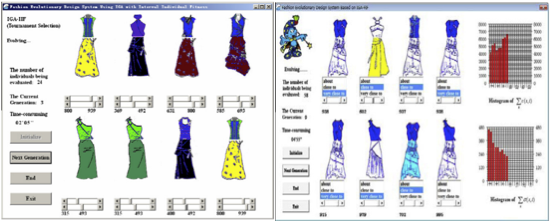
\includegraphics[width=10cm,height=10cm,keepaspectratio]{img/fashion.png}}
\caption{Different user interfaces interactive evolutionary system for fashion design.}
\label{fig:fashion}
\end{figure*}

\subsection{Web-Based IEC aplications .}


\subsubsection{Picbreeder.}
Picbreeder is a Web-based application that allows users to evolve images in a
collaborative way maintaining a large catalog of user-created content allowing
users collaboration by searching through extensive design spaces
\cite{secretan2008picbreeder}. Picbreeder provides to users of all
experience levels to enjoy all the creative contributions produced by other
users. In this way users experience a new form of recreation called creative
social recreation through collaborative exploration. In this sense these systems
helps their users to find interesting images through tagging, browsing and
searching as figure  \ref{fig:Picbreeder} show.

\begin{figure*}
\captionsetup{justification=centering,margin=2cm}
\centering
\setlength\fboxsep{0pt}
\setlength\fboxrule{0.7pt}
\fbox{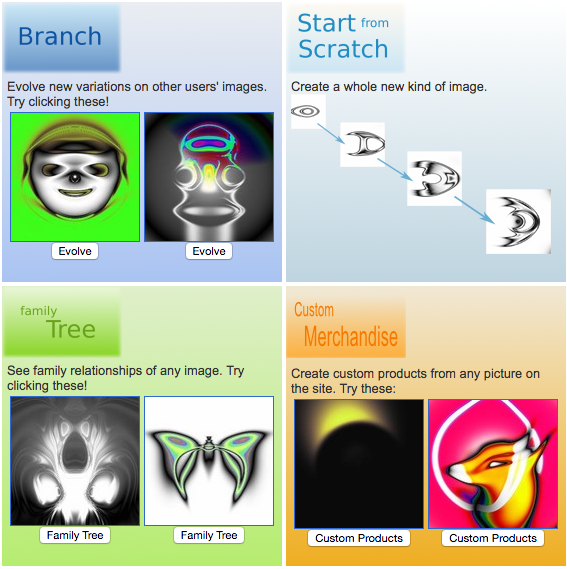
\includegraphics[width=10cm,height=10cm,keepaspectratio]{img/Picbreeder.png}}
\caption{Picbreeder User Selection.}
\label{fig:Picbreeder}
\end{figure*}

\subsubsection{EndlessForms.}
EndlessForms is a Web application that Explore object designs by choosing those
the users like. These selected objects become the parents of the next generation
of objects \cite{clune2011evolving}. EndLessForms proposes a new way to evolve
3D objects inspired by biological morphologies using generative encoding. One of
the experiments proposed in this paper was to use interactive evolutionary
systems to determine the potential for generating complex and interesting 3D
objects. They chose the interactive evolution, because that allows open-ended
exploration of the design space of objects that can produce by their method.
Additionally, the interactive evolution avoids the greedy nature of evolution by
objectives, which potentially allows to access more interesting objects
\cite{clune2011evolving}. In figure \ref{fig:EndlessForms} we can see some of
this objects.

\begin{figure*}
\captionsetup{justification=centering,margin=2cm}
\centering
\setlength\fboxsep{0pt}
\setlength\fboxrule{0.7pt}
\fbox{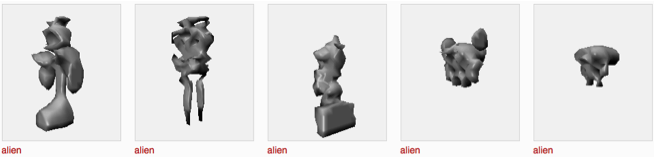
\includegraphics[width=10cm,height=10cm,keepaspectratio]{img/EndlessForms.png}}
\caption{Alien objects from EndLessForms.}
\label{fig:EndlessForms}
\end{figure*}

\subsubsection{EvoSpace-Interactive} EvoSpace-Interactive is an open source
framework focused on Web environments for collaborative interactive evolutionary
applications. This framework defines three main components for each application,
which are:
\begin{itemize}
	\item Individual.
	\item Processing Script.
	\item Worker Script.
\end{itemize}

The individual is represented internally as a data dictionary stored in Redis
[16] database management system; the individual contains main attributes as id,
chromosome, mom, dad, and views. This attributes represents the key information
of the individual as the individual offspring, the number of times that the
individual has been selected, etcetera, as shown in figure \ref{fig:individualRep} [3].

\begin{figure*}
	\captionsetup{justification=centering,margin=2cm}
	\centering
	\setlength\fboxsep{0pt}
	\setlength\fboxrule{0.7pt}
	\fbox{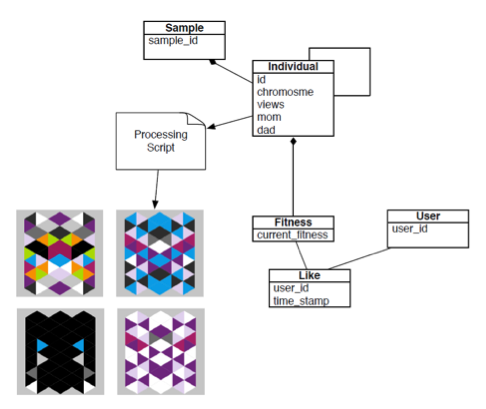
\includegraphics[width=10cm,height=10cm,keepaspectratio]{img/individualRep.png}}
	\caption{Individual Representation.}
	\label{fig:individualRep}
\end{figure*}

As we can observe on figure \ref{fig:ESFramework}, this work uses database
management systems to implement collaborative interactive evolutionary
applications. One of the reasons that this framework is using Redis[15] is
because it provides a hash- based implementation of sets and queues, which are
natural data structures for the EvoSpace model. On the other hand this framework
uses a relational database to save basic information about the user extracted
from the social platform (Facebook) through open graph API and OAuth2
authentication.
\begin{figure*}
	\captionsetup{justification=centering,margin=2cm}
	\centering
	\setlength\fboxsep{0pt}
	\setlength\fboxrule{0.7pt}
	\fbox{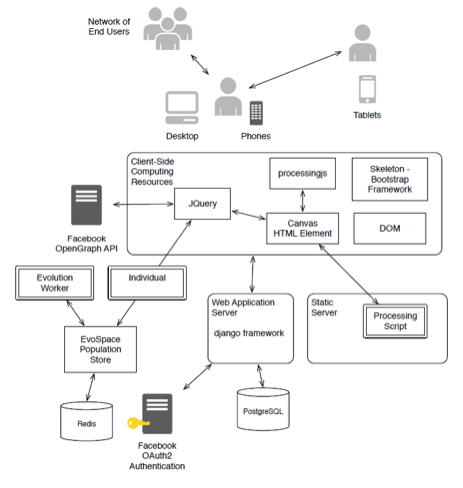
\includegraphics[width=10cm,height=10cm,keepaspectratio]{img/ESFramework.png}}
	\caption{EvoSpace-Interactive Framework.}
	\label{fig:ESFramework}
\end{figure*}

\section{User Modeling}

%%\subsection{Traditional Production Systems}

User modeling can be represented as the technique of building a model of the
user to personalize a system. The user model is commonly created as the user is
working with the system. An example is an educational application that teaches
students an individual skill: given the rules and knowledge in the user model,
the difficulty level of the exercises in the form is altered as the user
progresses.   Formally definition of user modeling according to McTear
\cite{mctear1993user} : " User modeling is the process of gathering information
about the users of a computer system and of using the information to provide
services or information adapted to the specific requirements of individual users
(or groups of users)". The purpose of the user model is to have a module
containing the operations that are needed to personalize the system, and the
user profile, which includes the personal data of the user
\cite{fischer2001user}. System personalization over user modeling is related
to the research field of adaptive systems; this subject is beyond the scope of
this research work. Focus on the human user, user modeling is a very
cross-disciplinary research topic, comprehending the domains of artificial
intelligence, computer science, and social science. Ideas have been co‐opted
from an extensive range of subdomains, such as human–computer interaction,
e‐learning, information science, social computing, machine learning, data
mining, cognitive science, and so on \cite{kay2012coming}
\cite{kobsa2001generic}. There is interest in user modeling from both a
scientific and commercial perspective \cite{razmerita2009user}.
\subsection{Application Domains for user modeling}

Amount Research and implementation exist in this domain in which personalization
and user modeling plays an important role. This section presents several works
of these domains. To understand this topic, the different objects are divided
into three general categories:
\begin{itemize}
	\item {supporting a user during a task. }
	\item {giving a user a specific personalized experience. }
	\item {training and educating a user.}
\end{itemize}
The categories especially differ in the kind of user data that is used. For each
domain, the general purpose of the domain and the more accurate purpose of the
user model are discussed.

\subsection{User models for providing task support}

Task support systems are f systems that help a user during a task by either
supporting the user perform the task or by completely taking over this task
\cite{brun2010compass}. For instance,  an application that
automatically categorizes the incoming emails of the user. The goal of the user
model in these requests is to promote the efficiency of interactions with the
user, to simplify these interactions and to make complex systems more usable
\cite{razmerita2009user}\cite{fischer2001user}.
To perform this personalization, data is
collected through observations of the user. This information is related to the
user’s goals and needs, but especially to the task that the user currently is
accomplished, like the user’s task knowledge and background. Much research has
been done in this domain, but because many separate research projects are
focusing on an exact task or subject, it is hard to make
generalizations or to establish one delimited investigation topic. Commonly
discussed research subjects are Decision Support Systems,  Adaptive Hypermedia,
and Adaptive Ubiquitous Systems, each having his or her own specific domain and
way of personalization.

\subsection{Decision support systems}

Decision support systems are systems that support a user with making a decision
in a complex, professional environment. For example,  a
system used at a pharmacy for automatically checking valid combinations of
medicine. The method can be used to help the pharmacist in prescribing the right
combinations and to give information for making a decision when a problem
occurs. The purpose of the user model in decision support systems is to present
the user with the right and appropriate information, giving different feedback
or applying various decision steps according to the characteristics of the
user.The data that is used is often associated with the user’s task and
background knowledge. The adaptation takes place by adapting the amount and
the content of the feedback provided by the system.


Decision support systems are traditionally ruled or logic-based systems, in
which all the relevant information is represented in a knowledge base. This
means that the content of the user model itself is also highly dependent on the
way the rules and knowledge are represented.


\subsection{Adaptive Hypermedia}

Adaptive hypermedia system is a system that grant users to browse freely
information network,  structured by nodes and links, to retrieve items of
information \cite{deepa2012adaptive}. For instance an internet website
application. The goal of the user model is to make the interface and structure
of the system dynamic. This enables the application to adapt to the user and to
make it easier for the user to search for and retrieve relevant information.
The data used in the user model is related to the user’s abilities, knowledge,
and goals in the application. The adaptation happens by adjusting the structure
and the presentation style to the expected needs of the user. For example, by
enhancing web search: promoting pages that might better correspond to the user’s
characteristics, on the other hand by giving navigation support, through
highlighting certain components of a page \cite{razmerita2012user}.

\subsection{User models for providing a personal experience.}

User models for providing the user with a personal experience have the goal to
improve the user experience while using the system.  This kind of user modeling
is especially focused on more commercial fields, such as e-commerce, marketing,
and computer games, and became popular with the rise of the Internet.  The
information that is used by the user in this main domain is mostly focused on
the information that defines the user, such as the user’s preferences and
interests. Since this data is regularly delicate, privacy is a  big issue
\cite{toch2012personalization}. While in others domains the privacy of the user
data is also important, in this area it is even a greater topic of discussion
because the incentive of the application developers is frequently contradictory
to the incentive of the actual user, considering gaining and sharing the user´s
personal information. For instance, user profiles are often shared among diverse
components of the same application, or even with different applications
\cite{brun2010compass} \cite{karam2012modeling}, which presents additional
weaknesses and possible undesirable information sharing.  Ensuring personal data
is not open to all people, in addition to defining strict privacy policies, is
thus essential in these user models. Some investigation in this domain are.

\subsection{Recommender Systems and User Adaptive Computer Games.}

Recommender systems are concerned with presenting the user with relevant
information and suggestions. They are commonly used on the Internet, for example
on websites such as Facebook, to provide the user with personalized news,
targeted advertisements and possibly new friends \cite{brun2010compass}. The
purpose of the user model is to give the system with information that is assumed
to be important for the user. The information that is stored for this goal is
associated with the preferences of the user to certain objects, like products,
music or people. To benefit a classification of these objects, the interaction
history of the user is stored, or the user is explicitly asked to rate certain
objects. The content of the system is eventually adjusted by showing the
recently inferred objects. In these senses, objects can be inferred by looking
at the attributes of the objects in the user profile, or by looking at the
objects in other user profiles that are related to the user \cite{kobsa2001generic}
\cite{kay2012coming}. As a result of the predominantly commercial target of these
systems, the adaptations often take place in a very invasive way, to make sure
the user notices the change. Most recommender systems are based on the Internet,
which means that some typical technical difficulties  are associated with these
kinds of user models. First, the user profile is often only stored while the
user’s visit,  which means that fast and efficient adaption is important.
Recommender systems usually become more precise  when the user spends more time
with the system. Second, the system’s architecture is usually client-server,
where the client side gathers user information and sends it to the server, where
the  actual process takes place.

\subsection{User Adaptive Computer Games.}

User Adaptive computer games are games that focus on increasing the perceived
value by providing a strongly individualized experience (Brisson, 2012).  For
example is a first‐person shooter that adapts the performance of the enemy
according to the shooting accuracy of the player.

The fundamental idea of the user model is to identify or classify the user, so
the appropriate adjustment is made in the computer game. The information that is
used addresses the preferences and progress of the user, such as the user´s
current  difficulty level or even the employed strategy. This data is usually
obtained through the interactions of  the user with the game, and therefor first
should be translated and formalized  before it can be  used to interpret
conclusions on a higher level. The adaptation that takes place in the game
concerns changing the content and role of the  game, such as the game
difficulty, the behavior of non‐player characters  or even the background  music
\cite{bakkes2012personalised}.

Because of the emphasis on the user, user adaptive computer games have
relatively a lot of processing power available  for personalization. In this
sense the user adaptive computer games domain is a very interesting research
domain.

\subsection{Adaptive Educational Games.}

Adaptive Educational Games (AEGs) are complicated educational games that combine
ideas from several investigations areas, to increase the student’s learning
experience \cite{peeters2012situated}. These are especially based on  serious
games: computer games with an educational approach, where things are taught to
students by using a  playful idea \cite{korteling2011transfer} \cite{johnson2005serious}.
For instance an AEG is a training application  for fire fighters, letting
the fire fighters train their skills and knowledge in a safe on a virtual
environment.

The objective of the user model in an AEGs is to optimize the learning process
and outcome.   The user information is considered with the advance and knowledge
of the student, but also with the  student’s mental and cognitive
characteristics. The gained data can be used to adjust the content,
presentation, and system behavior to the  student’s need, for example, by
adjusting the content, tone, or amount of presented feedback. Adaptive computer
games have a lot of processing power available for personalization,  making a
complex and interesting domain for user modeling.

\subsection{Methods for user modeling.}

In the user modeling topic, researchers have proposed more general design
methods and frameworks to guide the developers in the process of user modeling.
These general methods are useful in research projects, where the knowledge can
be reused to adjust the user model to the system’s characteristics. Also in
commercial applications, these general methods have proven to be useful
\cite{brun2010compass}, because they make it easier and more feasible to implement
personalization into a system. In early work, the process of user modeling was
mostly based on the intuition and experience of the developer or researcher. In
recent work, the techniques of user modeling were essentially based on the
intuition and expertise of the developer or researcher. As the user modeling
research field evolved, there has been put much effort in creating a general way
for designing and constructing a user model, by basing decisions on more
empirical grounds and by defining methods applicable to the whole field
\cite{kobsa2001generic} \cite{durrani1997cognitive}.

Frameworks, methodologies, and architectures have been developed, defining the
strict process, restrictions and choices on how to design and build a user
model. In the early days of user modeling, the focus was put on developing one
method applicable to the user modeling field as a whole. However, user modeling
is a very cross‐disciplinary research subject. Therefore, throughout the
decades, the user modeling area of research has been influenced by the important
research topics and trends of their time. For example, when information
technologies became a major subject in the early nineties, user modeling methods
were also mostly focused on the application of stereotypes, knowledge bases, and
logic to define a user model. With the rise of the Internet, the objectives of
the user modeling field change to Web-oriented applications and all the specific
problems that arise with this. Thus this connection,  also the general user
modeling methods that were developed, were focused on the popular research
domains of their time \cite{kay2012coming}. The main approaches to user modeling
did not change, but the specific filling‐in of the user model, such as which
technology to apply, did change. In this sense development of user modeling as a
whole, most researchers eventually agreed that one method to solve all problems
is not possible \cite{mctear1993user} \cite{kobsa2001generic}. Instead, a broad
range of  generic user modeling methods has been developed
\cite{fischer2001user}; each of which supports only a few of the very different
manifestations of personalization.



\section{Gamification.}

A definition given by Huotari  \cite{huotari2012defining} is  “Gamification is
the process by which concepts are brought to the real world task associated with
real people”. Also gamification handle game design elements which are commonly
known as non-game context in the pursue to  enhance user engagement,
organizational productivity, flow, learning, evaluations, among others.

Games and game technologies increase exponentially the traditional boundaries of
their medium, as evidenced by the growth of serious and pervasive games as an
industry and research field. The most recent phenomenon in this path is
‘gamification’, paradigm for the use of video game elements (rather than full-
fledged games) to improve user experience and user engagement in non-game
services and applications \cite{deterding2011gamification}.

\subsection{Techniques.}


Techniques in this context seek to persuade users to use their natural desire to
compete, learn and socialize in given non-game context application
\cite{deterding2011game}\cite{hamari2014does}. Some works in the beginning used
rewards for users as players to perform desired tasks in a certain application
or involving users to compete with each other. For instance some sort of
rewards include points \cite{sutter2010browse}, achievement badges or levels
\cite{hamari2011framework}, the filling of a progress bar \cite{o2010get}, or
providing the user with virtual currency. By Making the rewards for  tasks
achievements visible to other players or providing leader boards are ways of
encouraging players to compete \cite{hickman2010total}. Because the  problematic
consequences of competition, which can result in negative conduct, low
cooperation and collaboration, or disadvantaging certain player demographics
such as women \cite{kumar2013gamification}, best-practice gamification designs
try to refrain from using this element.

Another techniques to gamification is to make existing tasks feel more like
games \cite{deterding2010just}. Some techniques used in this approach include
adding meaningful choice, onboarding with a tutorial, increasing challenge, and
adding narrative \cite{mcgonigal2011reality}.
